\subsection{Gestión de Usuarios}

    Esta iteración tuvo como propósito implementar un mecanismo que permita a los usuarios del sistema autenticarse y/o crear cuentas
    para acceder al mismo, las actividades realizadas fueron:
    \begin{enumerate}
        \item Se diseñó e implementó las interfaces de usuario para la gestión de cuentas y accesos.
        \item Se especificaron los requerimientos mediante casos de uso con sus respectivas interfaces de usuario.
        \item Se elaboró el diagrama de casos de uso para este sprint.
        \item Se elaboró la máquina de estados de un reclutador.
    \end{enumerate} 

    Los requerimientos funcionales de este sprint se muestran en la siguiente tabla.
    \begin{requerimientos}{funcionales}
        \RFitem{RF-GRL-01}{Iniciar sesión}{El sistema debe proporcionar un mecanismo que permita al actor acceder al sistema mediante un correo y una contraseña.}
        \RFitem{RF-GRL-02}{Crear cuenta}{El sistema debe proporcionar un mecanismo que permita al actor registrarse como nuevo usuario en el sistema.}
        \RFitem{RF-USR-04}{Consultar perfil}{El sistema debe permitir al actor acceder a su perfil para consultar la información registrada.}
        \RFitem{RF-USR-05}{Editar perfil}{El sistema debe permitir al actor modificar la información registrada en su perfil, como nombre, apellidos, información de contacto y si el usuario es un candidato, debe de permitir modificar su información académica y datos de habilidades y conocimientos del mismo.}
        \RFitem{RF-EM-24}{Enviar solicitud para acceder al sistema}{El sistema debe proporcionar un mecanismo para que al representante de una empresa pueda enviar una solicitud o pre-registro de poder acceder y publicar vacantes.}
    \end{requerimientos}

    Los casos de uso que se describieron en este sprint pertenecen al \textbf{Módulo General (GRL)} el cual tiene como objetivo 
    permitir el acceso al sistema para todos los actores y al \textbf{Módulo de Usuarios (USR)} la configuración del perfil de usuario dentro del sistema.

    En la figura \ref{dcu:MUSR} se puede ver el diagrama de casos de uso del \textbf{Módulo de General (GRL)} y en la figura 
    \ref{dcu:CUPUSR} se puede ver el diagrama de casos de uso del \textbf{(GRL)}.
    \begin{itemize}
        \item Los casos de uso \IUazul{} , son aquellos que se van implementar en este sprint.
        \item Los casos de uso \IUblanco{}, se tienen planeados para sprints posteriores.
    \end{itemize} 

    \begin{figure}[H]
        \begin{center}
            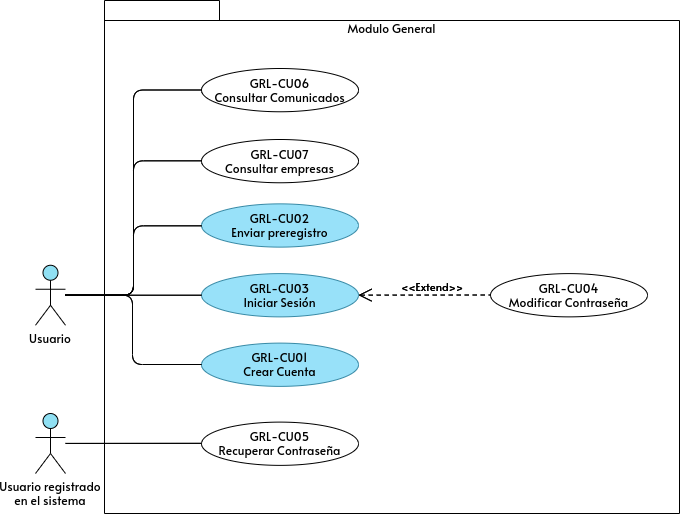
\includegraphics[width=.7\textwidth]{sprints/imagenes/CUGRL.png}
        \end{center}
        \caption{Diagrama de casos de uso del \textit{Módulo General}.}
        \label{dcu:MUSR}
    \end{figure}

    A continuación se listan los casos de uso de este sprint para el módulo general:
    \begin{itemize}
        \item \refElem{GRL-CU01}
        \item \refElem{GRL-CU02}
        \item \refElem{GRL-CU03}
    \end{itemize} 

    \begin{figure}[H]
        \begin{center}
            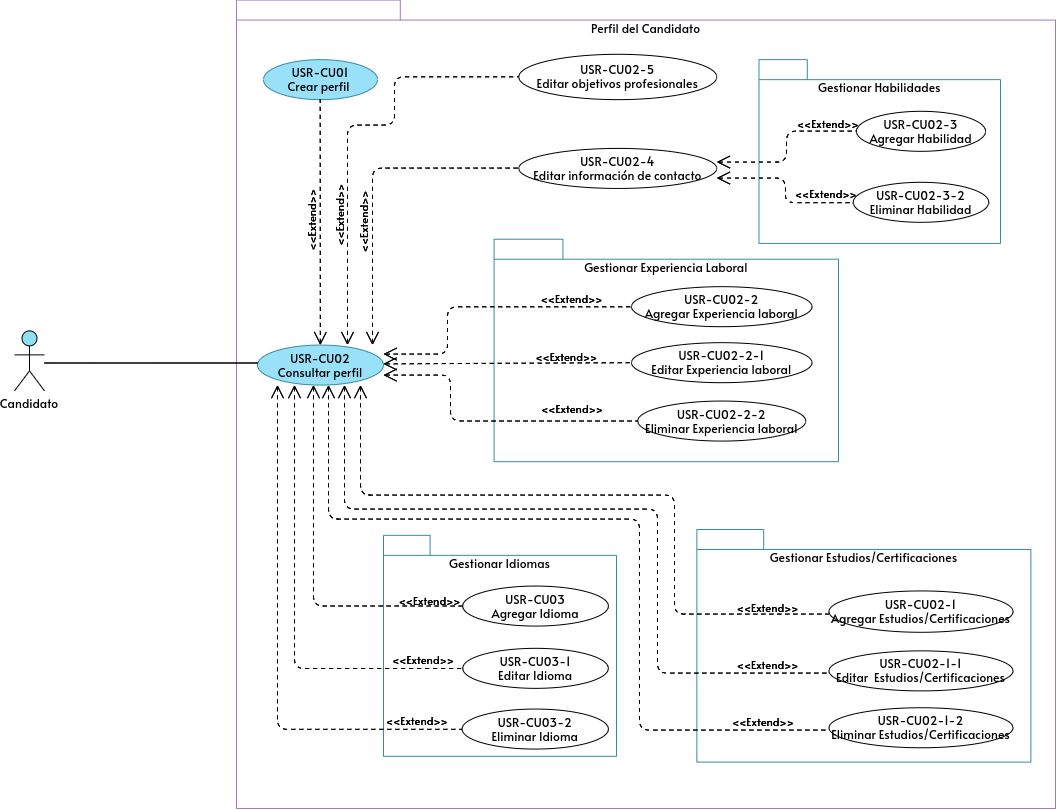
\includegraphics[width=.7\textwidth]{sprints/imagenes/CUPUSR.png}
        \end{center}
        \caption{Diagrama de casos de uso del \textit{Módulo de Usuarios}.}
        \label{dcu:CUPUSR}
    \end{figure}

    A continuación se listan los casos de uso de este sprint para el módulo de usuarios:
    \begin{itemize}
        \item \refElem{USR-CU01}
    \end{itemize} 

        El \textit{Módulo General} fue el primero en desarrollarse ya que permite conocer el tipo de usuario
        que está ingresando al sistema.\\ 
        \newline        
        En la construcción del módulo de inicio de sesión para los usuarios, se empleó el uso de JSON Web Token (JWT), este es un 
        estándar publicado en el RFC 7519 que nos permite el intercambio seguro de datos y nos facilita el proceso de determinar la 
        identidad de un usuario o autorizar a usuarios a realizar una acción.
        %En la figura  se muestra un diagrama de flujo en el que se describe el uso del Web Token en el sistema. 

        Al utilizar Django, se crea por defecto una tabla genérica llamada \textit{users} la cual nosotros seleccionamos
        la version por defecto minima, de esta forma pudimos utilizar las funciones del JSON Web Token y a su vez la modificamos 
        de tal forma que pudiéramos cubrir los requerimientos de este sprit.
        %\clearpage
        En la figura \ref{tbdb:users} se muestra la tabla \textit{users} tal como utiliza en el sistema. 
        \begin{figure}[H]
            \begin{center}
                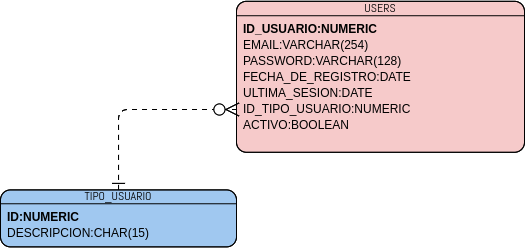
\includegraphics[width=.7\textwidth]{sprints/imagenes/sp1mdd.png}
            \end{center}
            
            \caption{Tabla \textit{users}.}
            \label{tbdb:users}
        \end{figure}
    
        Por parte del frontend necesitamos el uso de dos servicios con React js para administrar el JWT, el primer servicio es para realizar una petición HTTP con el verbo POST, teniendo como payload un objeto con los datos de correo electrónico y contraseña. Una vez realizada la petición HTTP al servidor, se asignará un token de acceso y un token de actualización, el token de acceso nos ayudará para identificar si el usuario en cuestión tiene los permisos para acceder a un determinado recurso dentro del sistema o para realizar una consulta de información a la API. Por otro lado, el token de actualización es por motivos de seguridad, ya que los tokens de acceso tienen un ciclo de vida corto y una vez que caducan, la aplicación del lado del cliente puede hacer uso del token de actualización para actualizar el token de acceso, es decir, los tokens de actualización nos permite obtener nuevos tokens de acceso sin tener que pedirle al usuario que inicie sesión nuevamente.\\
        \newline
        Hasta este punto, ya tenemos nuestros tokens y podemos iniciar sesión, un problema que se presentó fue en el momento de refrescar el navegador, ya que la sesión del usuario no persistía, una solución propuesta fue usar un segundo servicio que se encargará de interceptar la llamada a la API que nos genera los tokens, esto porque debemos saber si el token de acceso ha caducado se realice una nueva solicitud para obtener un nuevo token, el cual se le asigna a la petición original y de esta forma el usuario tendrá un token actualizado.\\
        \newline        
        Mientras tanto en el backend se valida que el payload de las credenciales enviadas por el frontend pertenezcan a un usuario activo en la base de datos. Para el manejo de los usuarios se usaron las capacidades de la tabla “Users” disponible en Django por defecto, con los campos mínimos que posee por defecto y agregando campos propios, ya que esta tabla cuenta con las funciones de seguridad integradas necesarias para encriptar contraseñas y validar la información recibida por el frontend y empezar el intercambio de tokens entre ambas partes de forma segura. Con la generación e intercambio de tokens funcionando correctamente se implementó el uso de las tablas de los usuarios definidos por el modelado de datos utilizando una representación de especiación, siendo la tabla “Users” la tabla de usuarios en general, posteriormente en las tablas de los usuarios del sistema se hace referencia a la llave primaria del registro propio del usuario en “Users” para consultar la información del usuario y pueda hacer uso de la plataforma.
        
       